\documentclass{article}

\usepackage[hyphens]{url} 


\usepackage[utf8]{inputenc}

\usepackage{pdfpages}
\usepackage{lastpage}
\usepackage{fancyhdr}
\usepackage{ngerman}
\usepackage{listings}
\usepackage{hyperref}
\usepackage{tabularx}
\usepackage{floatrow}
\usepackage[tableposition=top]{caption}
\floatsetup[table]{capposition=top}

\usepackage{amsmath, amssymb}
\usepackage{multirow}
\usepackage[utf8]{inputenc}

\usepackage{xifthen}
\usepackage[numbib]{tocbibind}

\newcommand\twodigits[1]{%
   \ifnum#1<10 0#1\else #1\fi
}



\lhead{Phase und Leistung}
\rhead{27. November 2020\\T. Maier, J. Winkler}
%\cfoot{\twodigits{\thepage}~/ \pageref{LastPage}}
\cfoot{{\thepage}~/ \pageref{LastPage}}

\newcommand{\W}{\text{W}}
\newcommand{\V}{\text{V}}
\newcommand{\A}{\text{A}}

\newcommand{\UR}{$U_R$ }
\newcommand{\UIR}{$U_\text{IR}$ }

\newcommand{\mini}{\operatorname{min}}



\definecolor{commentgreen}{RGB}{2,112,10}
\definecolor{eminence}{RGB}{108,48,130}
\definecolor{weborange}{RGB}{255,165,0}
\definecolor{frenchplum}{RGB}{129,20,83}

\lstdefinelanguage{python}{
    morekeywords={def, for, range, abs, return},
    otherkeywords={<-,->, |>, \%\{, \}, \{, \, (, )},
    sensitive=true,
    morecomment=[l]{\#},
    morecomment=[n]{/*}{*/},
    morecomment=[s][\color{purple}]{:}{\ },
    morestring=[s][\color{orange}]"",
    commentstyle=\color{commentgreen},
    keywordstyle=\color{eminence},
    stringstyle=\color{red},
	basicstyle=\ttfamily,
	breaklines,
	showstringspaces=false,
	frame=tb
}
\lstset{
extendedchars=\true,
inputencoding=utf8
}




\begin{document}

\parindent0cm

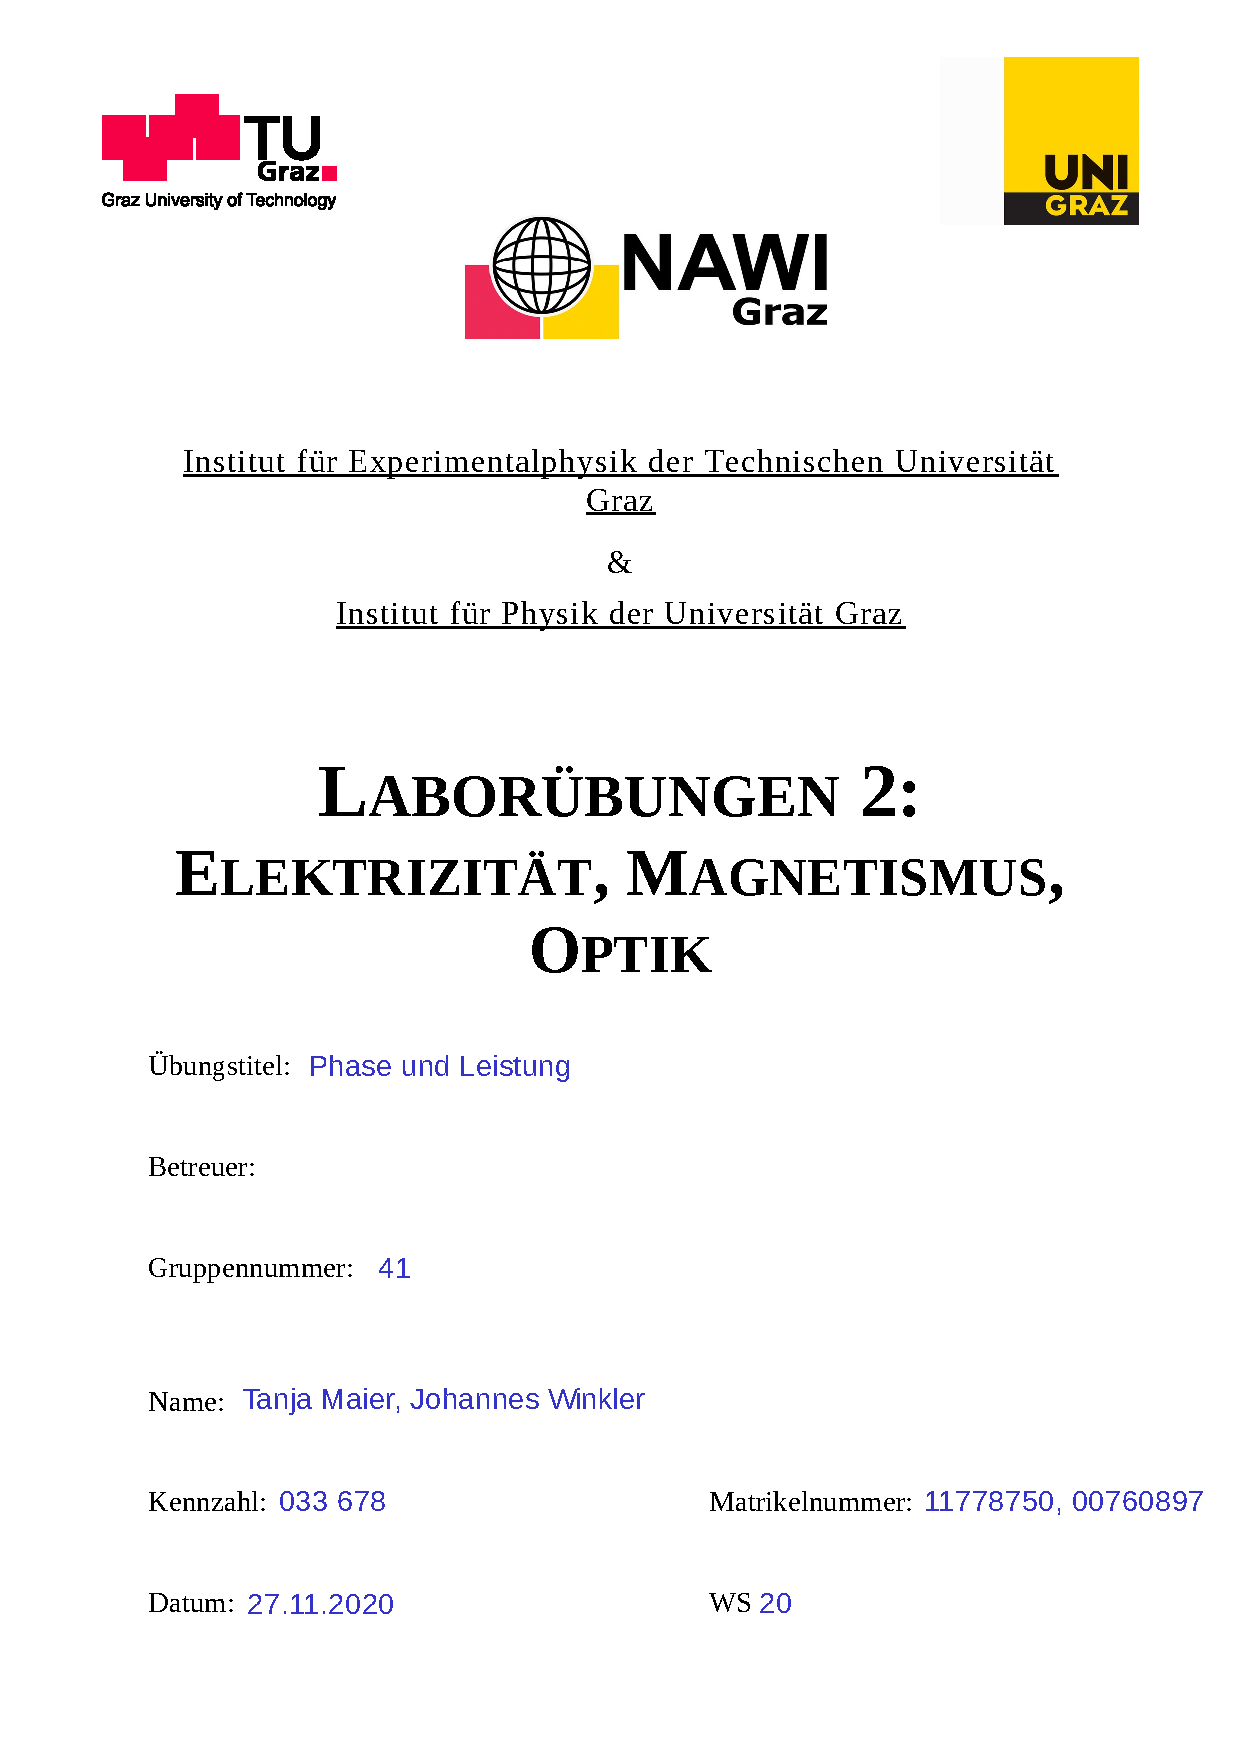
\includepdf{Deckblatt.pdf}


\pagestyle{fancy}

\tableofcontents
\newpage
\section{Aufgabenstellung}

\begin{enumerate}
\item Untersuchung  der  Anzeige  von  unterschiedlichen  Spannungsmessinstrumenten  bei verschiedenen Kurvenformen.
\item Messtechnische Ermittlung der Phasenlage von Strom und Spannung an einem Kondensator.
\item Messtechnische Ermittlung der Phasenlage von Strom und Spannung an einer Spule.
\item Messtechnische Ermittlung der elektrischen Leistung in einer RC-Schaltung.
\item Messtechnische Ermittlung der elektrischen Leistung in einer RL-Schaltung.
\end{enumerate}

\section{Voraussetzungen und Grundlagen}

\subsection{Wechselstrom und Wechselspannung}

Als Wechselstrom bezeichnet man jene Art von elektrischem Strom, bei der sich die Stärke und die Richtung periodisch ändern. Damit einhergehend ändert sich auch die Spannung und wird daher als Wechselspannung bezeichnet. Wichtige Größen sind hier der Scheitelwert (Maximalbetrag des Augenblickwertes bei einem Wechselsignal) und die sogenannten Effektivwerte $I_\text{eff}$ und $U_\text{eff}$. Dies sind jene Werte, bei denen im Wechselstromkreis die gleiche Leistungsabgabe, wie beim Gleichstromkreis (also keine periodische Änderung von Stärke und Richtung des Stroms) mit denselben Werten erfolgt.
\begin{align}
U_\text{eff} &= \sqrt{ \frac{1}{\tau}\cdot \int_0^\tau u^2(t)\cdot dt } \\ I_\text{eff} &= \sqrt{ \frac{1}{\tau}\cdot \int_0^\tau i^2(t)\cdot dt }
\end{align}
dabei ist $u(t)$ der Augenblickswert der Spannung, $i(t)$ der Augenblickswert des Stroms und $\tau$ die Periodendauer des Signals.
Zudem kann aus diesen Größen auch der Scheitelfaktor berechnet werden, der das Verhältnis von Scheitelwert zu Effektivwert (sowohl für Strom als auch für Spannung) darstellt.
\begin{align}
f_s &= \frac{U_s}{U_\text{eff}} \\
f_s &= \frac{I_s}{I_\text{eff}} 
\end{align}
Ähnlich zum Effektivwert lässt sich auch der Gleichrichtwert für Strom und Spannung als zeitliches Mittel berechnen
\begin{align}
U_\text{gl} &= \frac{1}{\tau}\cdot \int_0^\tau \left|u(t)\right|\cdot dt  \\ I_\text{gl} &= \frac{1}{\tau}\cdot \int_0^\tau \left|i(t)\right|\cdot dt 
\end{align}
Der Formfaktor (Verhältnis von Effektivwert zu Gleichrichtwert) ergibt sich dann als
\begin{align}
f_f &= \frac{U_\text{eff}}{U_\text{gl}} \\
f_f &= \frac{I_\text{eff}}{I_\text{gl}} 
\end{align}
Wichtig zu beachten ist, dass Scheitelfaktor und Formfaktor vom zeitlichen Verlauf des Signals abhängen dementsprechend unterschiedliche Werte liefern. (vgl. \cite{moodle}, \cite{src2}, \cite{src3}, \cite{src4}, \cite{src5})


\subsection{Messung von Gleichrichtwert und Effektivwert}

Um den Gleichrichtwert bestimmen zu können wird zunächst eine Gleichrichterschaltung aufgebaut und mithilfe dieser kann dann der Betrag der elektrischen Größe gebildet werden. Durch Einsetzen eines Tiefpassfilters erhält man auch das zeitliche Mittel.

Der Zusammenhang zwischen berechnetem Mittelwert und Scheitelwert der Wechselspannung ist gegeben durch

\begin{align*}
\left|\overline{U}\right| = ... = \frac{2}{\pi}\cdot \hat{U}
\end{align*}

Bei sinusförmigen Kurven kann hier außerdem noch ein Korrekturwert von $K_{\sin} = \dfrac{\pi}{2\cdot \sqrt{2}} \approx 1.11$ miteinbezogen werden, der sich aus dem Verhältnis vom Mittelwert des Betrags zum tatsächlichen Effektivwert der Spannung ergibt. Diese Messung des Effektivwertes mithilfe des Mittelwerts funktioniert jedoch nur bei sinusförmigen Signalen.

Für beliebige Signale werden andere Methoden verwendet, wie z. B. die termische Umformung, bei der ein Widerstand durch die Wechselgröße aufgeheizt wird. Die Temperatur, die erreicht wird, dient dann als Richtwert für einen zweiten Widerstand, der über einen Gleichstrom erhitzt wird. Beim Temperaturgleichstand wird dann auch die gleiche Leistung umgesetzt. Somit gilt $U_\text{eff} = U_\text{RMS}$ bzw. $I_\text{eff} = I_\text{RMS}$. (vgl. \cite{moodle}, \cite{src3}, \cite{src5})


\subsection{Wechselstromwiderstände und deren Leistung}

Hierbei wird unterschieden zwischen Wirkleistung, Blindleistung und Scheinleistung. Die Wirkleistung ist jener Teil der Leistung, der in mechanische Arbeit umgewandelt wird. In einem Wechselstromkreis erfolgt hier eine Umwandlung von elektrischer in thermische Energie. Die Wirkleistung kann durch
\begin{align}
P = U\cdot I \cdot \cos(\phi)
\end{align}
beschrieben werden, wobei $U$ die Spannung und $I$ der Strom ist. $\phi$ ist die Phasenverschiebung. Man erkennt relativ leicht, dass die Leistung maximal wird, wenn die Phasenverschiebung gleich 0 ist ($\cos(0)=1$). (vgl. \cite{moodle}, \cite{src6})


Die Blindleistung wird zum Aufbau bzw. zum Abbau von elektromagnetischen Feldern benötigt und ergibt sich aus
\begin{align}
Q = U\cdot I \cdot \sin	(\phi)
\end{align}
wobei diese bei einer Phasenverschiebung von $\dfrac{\pi}{2}$ maximal wird.(vgl. \cite{moodle}, \cite{src6})


Die Scheinleistung ist die Gesamtleistung, die sich aus Wirkleistung und Blindleistung ergibt. Sie ergibt sich durch vektorielle Addition von $P$ und $S$
\begin{align}
S = P^2 + Q^2 = U\cdot I 
\end{align}




\section{Geräteliste}

\begin{table}[H]
\caption{Liste der verwendeten Geräte}

~

\begin{tabular}{l|p{2.3cm}p{3cm}lll}
Abk. & Gerätename    &  Modell/Wert  & Unsicherheit\\
\hline
N & Netzgerät & Hameg HM8040-2 \\
FG & Funktions\-generator & Hameg HM8030-3 \\
OS & Oszilloskop & DSO-X 2002A  & 2\% (vgl. \cite{oszi_datenblatt}) \\
MM1 & Multimeter (digital) & TTi 1604 & 0.5\% + 4 digits (vgl. \cite{moodle})\\
MM2 & Multimeter & M4600 & 0.5\% + 10 digits (vgl. \cite{moodle}) \\
MM3 & Multimeter & Unigor 4n & 1.5\% (vgl. \cite{moodle} \\
MM4-6 & Multimeter (digital) & Fluke 175 & 1\% + 3 digits \\
WM & Wattmeter & HM8115-2 \\
R & Widerstand & $R=68.0~\Omega$ & $\Delta R = 3.4~\Omega$ \\
C1 & Kondensator & $C_1=100~\mu$F & $\Delta C_1 = 20~\mu$F \\
C2 & Kondensator & $C_2=47~\mu$F & $\Delta C_2 = 10~\mu$F \\
C3 & Kondensator & $C_3=20~\mu$F & $\Delta C_3 = 4~\mu$F \\
C4 & Kondensator & $C_3=10~\mu$F & $\Delta C_3 = 2~\mu$F \\
\end{tabular}
\end{table}

Die Bezeichnungen MM1, MM2 und MM3 entsprechen den Geräten P1, P2 und P3 im Schaltplan von Aufgabe 1. In späteren Plänen ändern sich die Bezeichnungen im Schaltplan, sodass wir zum Zwecke der Eindeutigkeit diese Geräte mit MM1 bezeichnet haben. Das Messgerät MM4 (Fluke 175) liegt mehrfach vor, die weiteren Geräte werden als MM5 und MM6 bezeichnet.

Sämtliche Daten wurden nach den Versuch mit Python3.8 ausgewertet, wobei für Grafiken die Library \texttt{Matplotlib} verwendet wird. 





\section{Beschreibung der Versuchsanordnung}


\subsection{Untersuchung  der  Anzeige  von  unterschiedlichen  Spannungsmessinstrumenten  bei verschiedenen Kurvenformen}
\label{subsec:aufbau_task1}

Der Hameg HM8030-3 Funktionsgenerator wird verwendet um verschiedene Spannungskurven zu erzeugen. Der Ausgangswiderstand des Funktionsgenerators beträgt 50~$\Omega$. Die Frequenz wird auf 50~Hz gestellt. Dann wird die Spannung einmal mit dem Oszilloskop gemessen (inkl. Spitze-Spitze-Wert und Effektivwert). Zusätzlich werden noch 3 weitere Messgeräte (TTi1604, M4600 und Unigor 4) zur Messung der Spannung parallel geschalten. Die Messung der Effektivwerte soll verglichen werden.


\begin{figure}[H]
\centering
\caption{Versuchsaufbau, Aufgabe 1}
\label{fig:aufbau_task1}
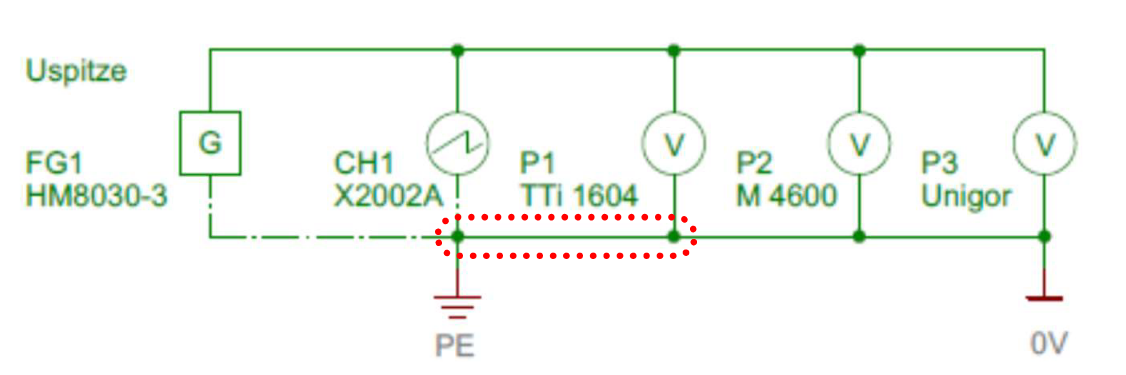
\includegraphics[scale=1]{bilder/aufbau_task1.png}
\end{figure}


\subsection{Phasenlage von Strom und Spannung an einem Kondensator bzw. einer Spule}

In diesem Versuch wird zweimal derselbe Versuchsaufbau verwendet, wobei der Kondensator für den dritten Versuch durch eine Spule ersetzt wird. Die Aufbauten sind in Grafiken~\ref{fig:aufbau_task2} und \ref{fig:aufbau_task3} zu sehen. CH2 misst die betreffende Spannung an Kondensator bzw. Spule, während CH1 für die Berechnung des dazugehörigen Stromes herangezogen wird.

Für das Signal wird in beiden Fällen ein Transformator herangezogen. Als Bezugspunkt für die Messung der Spannung wird in beiden Fällen das Verbindungsstück zwischen dem Widerstand und dem zu vermessenden Bauteil definiert.

\begin{figure}[H]
\centering
\caption{Versuchsaufbau, Aufgabe 2}
\label{fig:aufbau_task2}
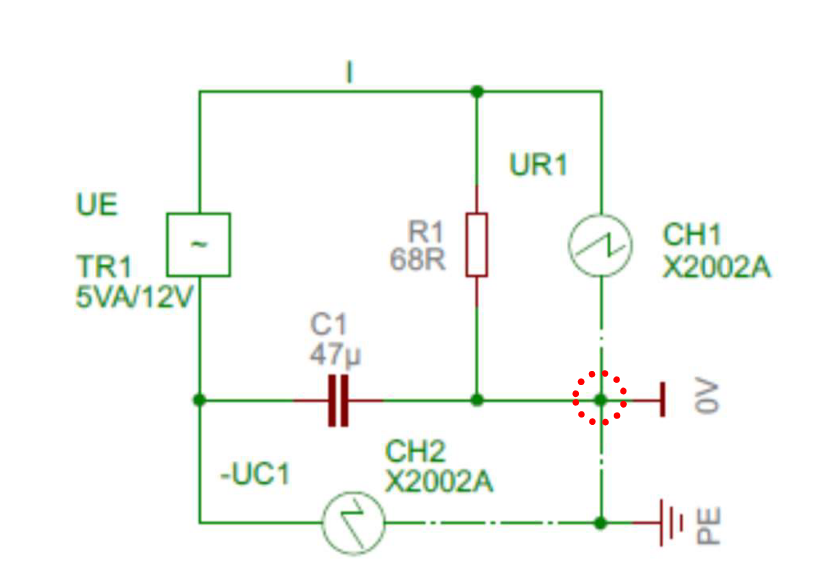
\includegraphics[scale=1]{bilder/aufbau_task2.png}
\end{figure}



\begin{figure}[H]
\centering
\caption{Versuchsaufbau, Aufgabe 3}
\label{fig:aufbau_task3}
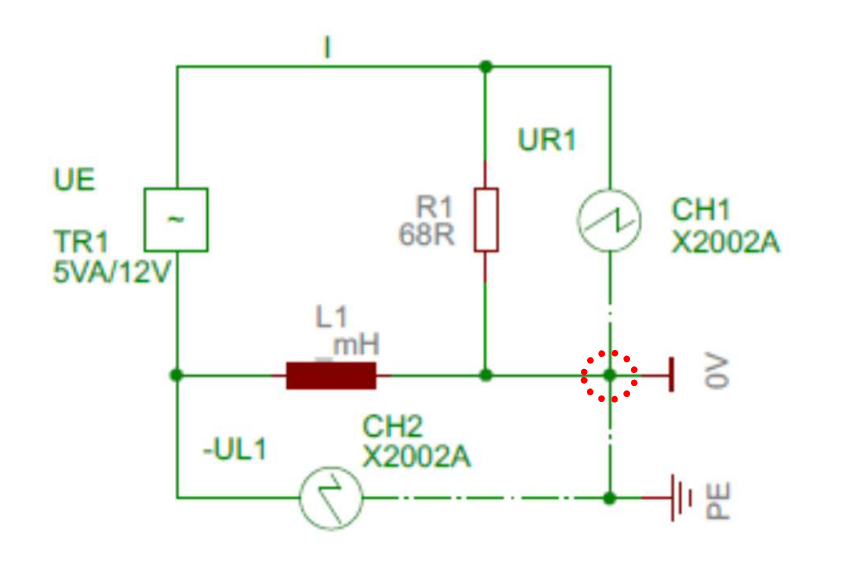
\includegraphics[scale=1]{bilder/aufbau_task3.png}
\end{figure}


\subsection{Leistung einer RC- bzw RL-Schaltung}

In diesem Kapitel ist die Leistung einer RC- bzw. RL-Schaltung zu bestimmen. Diese Schaltungen sind in den Grafiken~\ref{fig:aufbau_task4} und \ref{fig:aufbau_task5} dargestellt. Der Aufbau ist im wesentlichen identisch, bis auf den Kondensator in \ref{fig:aufbau_task4} und der Spule in \ref{fig:aufbau_task5}.



\begin{figure}[H]
\centering
\caption{Versuchsaufbau, Aufgabe 4}
\label{fig:aufbau_task4}
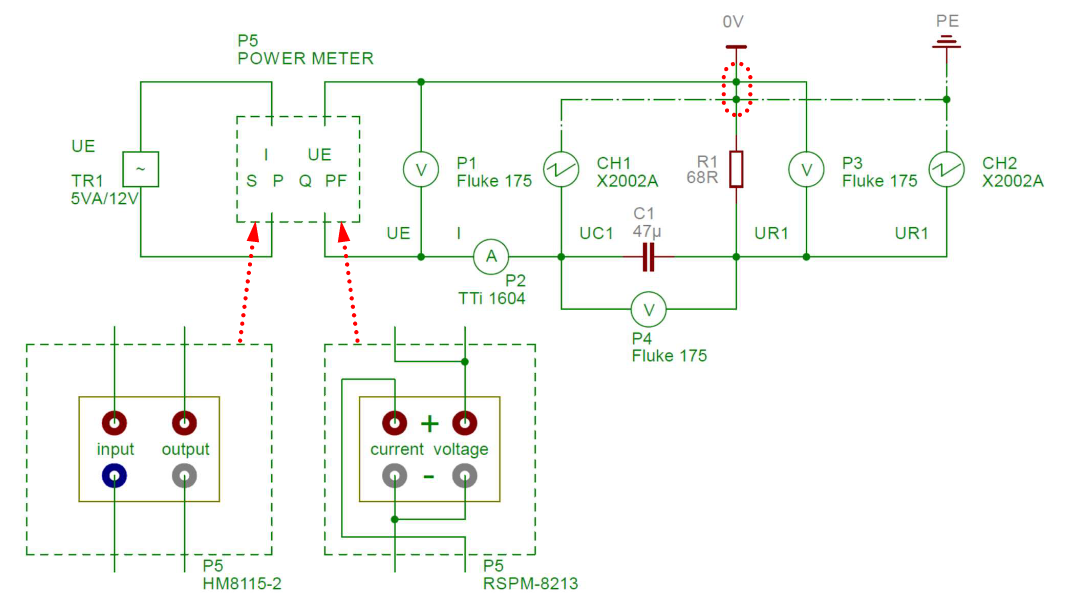
\includegraphics[scale=1]{bilder/aufbau_task4.png}
\end{figure}



\begin{figure}[H]
\centering
\caption{Versuchsaufbau, Aufgabe 5}
\label{fig:aufbau_task5}
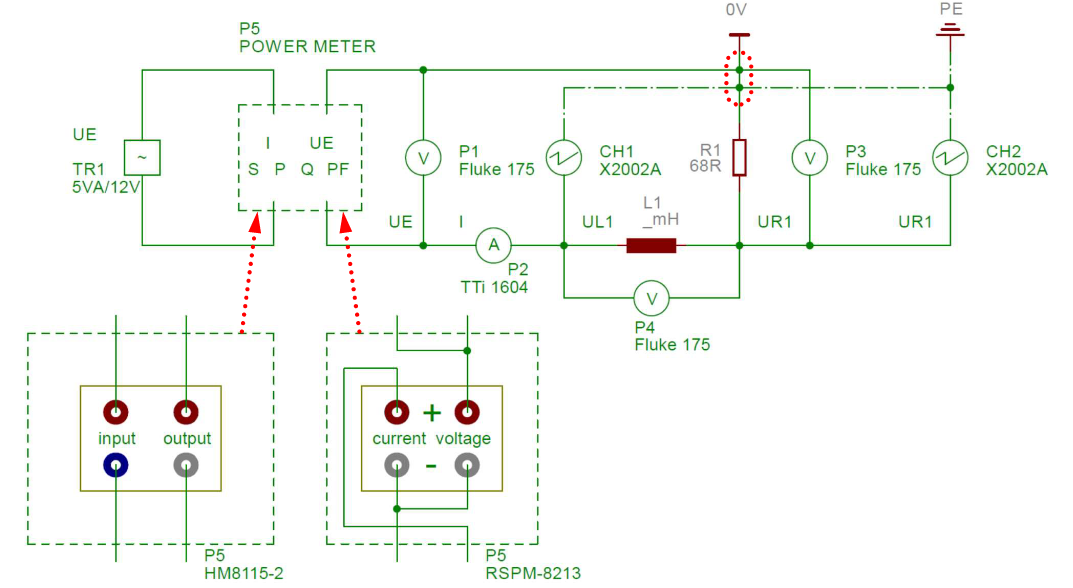
\includegraphics[scale=1]{bilder/aufbau_task5.png}
\end{figure}




\section{Versuchsdurchführung und Messwerte}

\subsection{Untersuchung  der  Anzeige  von  unterschiedlichen  Spannungsmessinstrumenten  bei verschiedenen Kurvenformen}

Abschnitt~\ref{subsec:aufbau_task1} beschreibt den Aufbau des Versuchs. Dieser wird nun mit einer Sinusspannung, einer Dreiecksspannung und einer Rechtecksspannung durchgeführt. Diese Kurven sollten jeweils dieselbe Frequenz und Amplitude haben, um die Ergebnisse besser vergleichen zu können. Das Oszilloskop zeichnet diese 3 Kurven. Sie sind in Grafiken \ref{fig:task1_sin}, \ref{fig:task1_dreieck} und \ref{fig:task1_rechteck} dargestellt. Zusätzlich wurde der Effektivwert mit 3 verschiedenen Messgeräten gemessen und soll verglichen werden.


\begin{figure}[H]
\centering
\caption{Sinusschwingung für Aufgabe 1}
\label{fig:task1_sin}
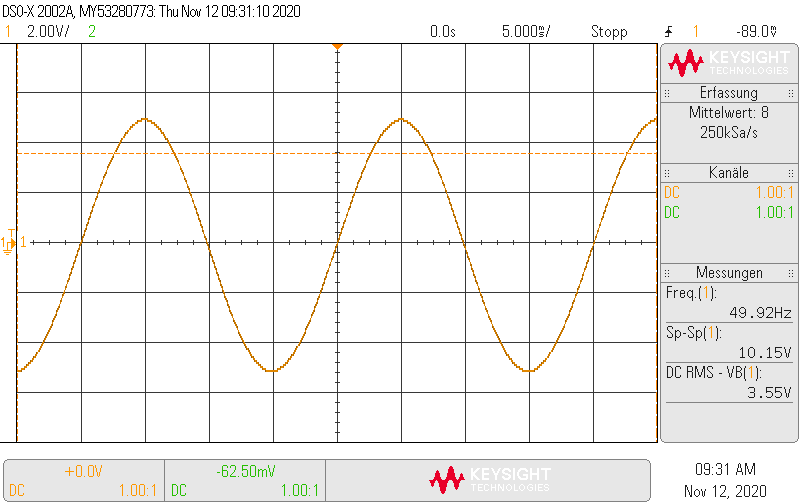
\includegraphics[scale=0.4]{daten/pul_1.png}
\end{figure}

\begin{figure}[H]
\centering
\caption{Dreiecksschwingung für Aufgabe 1}
\label{fig:task1_dreieck}
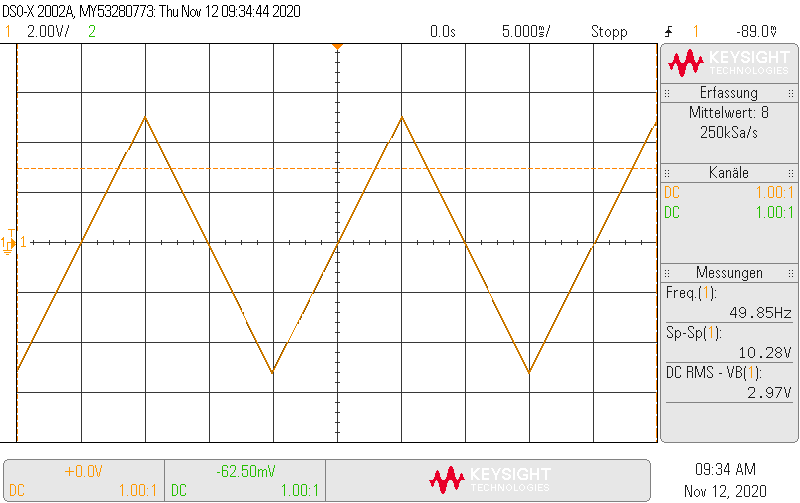
\includegraphics[scale=0.4]{daten/pul_2.png}
\end{figure}

\begin{figure}[H]
\centering
\caption{Rechtecksschwingung für Aufgabe 1}
\label{fig:task1_rechteck}
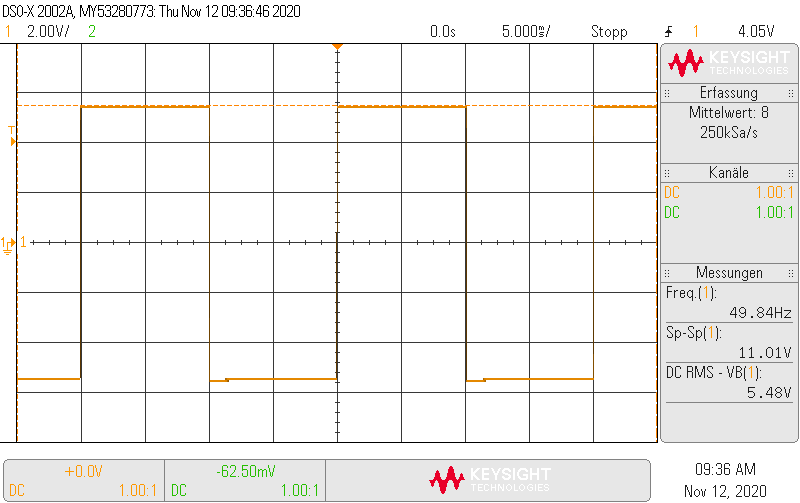
\includegraphics[scale=0.4]{daten/pul_3.png}
\end{figure}


Die gemessenen Werte werden in Tabellen~\ref{tab:messung_task1_volt} und~\ref{tab:messung_task1_oszi} zusammengefasst.

\begin{table}[H]
\centering
\caption{Gemessene Effektivwerte im Versuch 1 mit 3 verschiedenen Messgeräten. $U_1$ ist MM1 (P1 laut Schaltplan), $U_2$ ist MM2 (P2 laut Schaltplan) und $U_3$ ist MM3 (P3 laut Schaltplan). Alle Unsicherheiten sind aus den Datenblättern entnommen und in der Geräteliste angegeben.}
\label{tab:messung_task1_volt}
\begin{tabular}{r|rrr}
& P1 & P2 & P3 \\
Schwingung & $U_{1,\text{eff}}$ / V  & $U_{2,\text{eff}}$ / V & $U_{3,\text{eff}}$ / V \\
\hline
Sinus & $3.532\pm 0.022$ & $3.535 \pm 0.028$ & $3.31 \pm 0.05$ \\
Dreieck & $2.965\pm 0.019$ & $2.863 \pm 0.024$ & $2.66 \pm 0.04$ \\
Rechteck & $5.500\pm 0.032$ & $6.003 \pm 0.040$ & $5.91 \pm 0.09$
\end{tabular}
\end{table}


\begin{table}[H]
\centering
\caption{Messwerte bei Versuch 1 mit Oszilloskop. Alle Unsicherheiten sind in der Geräteliste angegeben.}
\label{tab:messung_task1_oszi}
\begin{tabular}{r|rr}
Schwingung &  $U_{ss}$ / V &  $U_\text{eff}$ / V  \\
\hline
Sinus & $10.15 \pm 0.20$ & $3.55 \pm 0.07$ \\
Dreieck & $10.28 \pm 0.21$ & $2.97 \pm 0.06$ \\
Rechteck & $11.01 \pm 0.22$ & $5.48 \pm 0.11$
\end{tabular}
\end{table}



\subsection{Phasenlage von Strom und Spannung an einem Kondensator bzw. einer Spule}

In diesem Fall werden beide Versuchsaufbauten (Grafiken~\ref{fig:aufbau_task2} und \ref{fig:aufbau_task3}) vermessen und man erhält die jeweiligen Kurven. Diese sind in Grafiken~\ref{fig:task2_kurve} und \ref{fig:task3_kurve} zu sehen. Gemäß der jeweiligen Versuchsaufbauten ist CH1 proportional zu den Strom durch Spule bzw. Kondensator. Man erkennt in Grafik~\ref{fig:task2_kurve} deutlich, dass der Strom (CH1) der Spannung (CH2) vorausgeht. Bei der Spule in Grafik~\ref{fig:task3_kurve} ist es genau umgekehrt.

\begin{figure}[H]
\centering
\caption{Kurve des Kondensators aus Aufgabe 2}
\label{fig:task2_kurve}
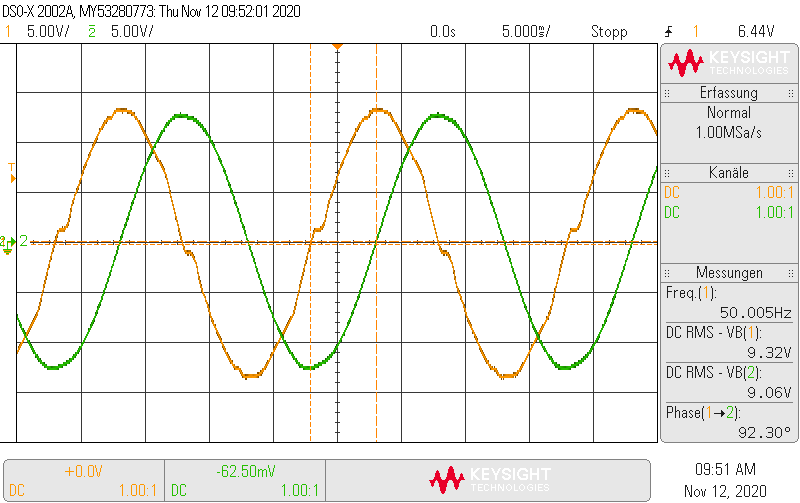
\includegraphics[scale=0.4]{daten/pul_4.png}
\end{figure}

\begin{figure}[H]
\centering
\caption{Kurve der Spule aus Aufgabe 3}
\label{fig:task3_kurve}
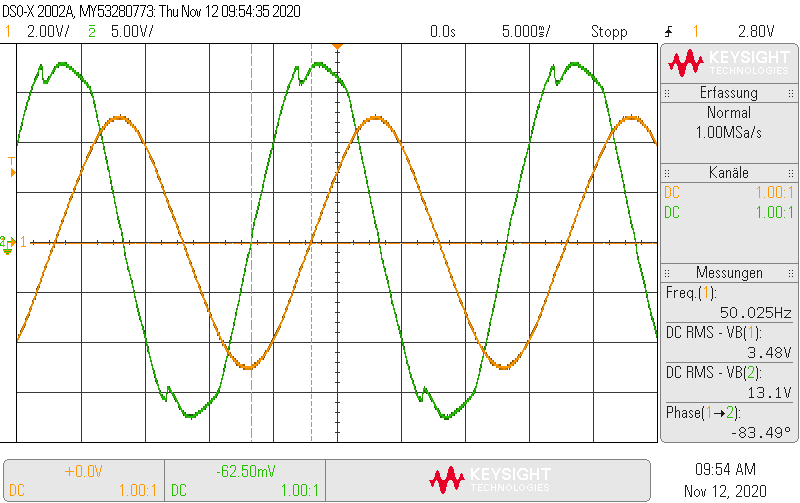
\includegraphics[scale=0.4]{daten/pul_5.png}
\end{figure}


\subsection{Leistung einer RC- bzw RL-Schaltung}

In diesem Teil werden die Daten für die Berechnung der Leistungsaufnahme einer RC- bzw RL-Schaltung gemessen. Für die Messung der Leistung sind sowohl die Eingangsspannung $U_E$, der Strom $I$, sowie die Phasenverschiebung nötig.

Das Wattmeter wird zwischen Transformator und RC/RL-Schaltung geschaltet. Dadurch können die Größen in Tabelle~\ref{tab:task45_wattmeter} ermittelt werden. Diese Werte liefern die Leistungsaufnahme der Schaltung. 

\begin{table}[H]
\caption{Werte des Wattmeters WM (P5 laut Schaltplan) für die RC bzw. RL Schaltung in den Versuchen 4 und 5}
\label{tab:task45_wattmeter}

\begin{tabular}{c|rrrrrr}
& $U_E$ / V & $I$ / A & $P$ / W & $Q$ / W & $S$ / W & $\cos(\phi)$ \\
\hline 
RC & 13.3 & 0.137 & 1.342 & 1.22 & 1.182 & 0.74 \\
RL & 13.9 & 0.051 & 0.256 & 0.65 & 0.699 & 0.37
\end{tabular}
\end{table}





Zusätzlich befinden sich 3 Messgeräte vom Typ Fluke 175 (MM4, MM5 und MM6 laut Geräteliste, P1, P3, P4 laut Schaltplan) in der Schaltung zur Messung von Spannungen. Für die Messung des Stromes wird ein TTi 1604 (MM1 laut Geräteliste, P2 laut Schaltplan) verwendet. Diese Messungen wurden zusätzlich durchgeführt und in Tabelle~\ref{tab:task45_messungen} aufgelistet.


\begin{table}[H]
\caption{Händisch durchgeführte Messungen mit P1, P2, P3 und P4 laut Schaltplan. Messungen jeweils für RC und RL Schaltung.}
\label{tab:task45_messungen}

\begin{tabular}{c|rrrrr}
& P1 & P2 & P3 & P4 & P4 \\
& $U_E$ / V & $I$ / mA & $U_{R1}$ / V & $U_{C1}$ / V & $U_{L1}$ / V \\
\hline 
RC & 13.24 & 136.7 & 9.19 & 8.97 & -- \\
RL & 13.83 & 51.0 & 3.41 &  -- & 13.07
\end{tabular}
\end{table}




Bei den Versuchsaufbauten in Grafik \ref{fig:aufbau_task4} und \ref{fig:aufbau_task5} wird jeweils mit dem Oszilloskop die Spannung an zwei Stellen gemessen. Diese Spannungen sind für die RC-Schaltung in Grafik~\ref{fig:task4_kurve}, und für die RL-Schaltung in Grafik~\ref{fig:task5_kurve} dargestellt.



\begin{figure}[H]
\centering
\caption{Spannungen in einer RC-Schaltung}
\label{fig:task4_kurve}
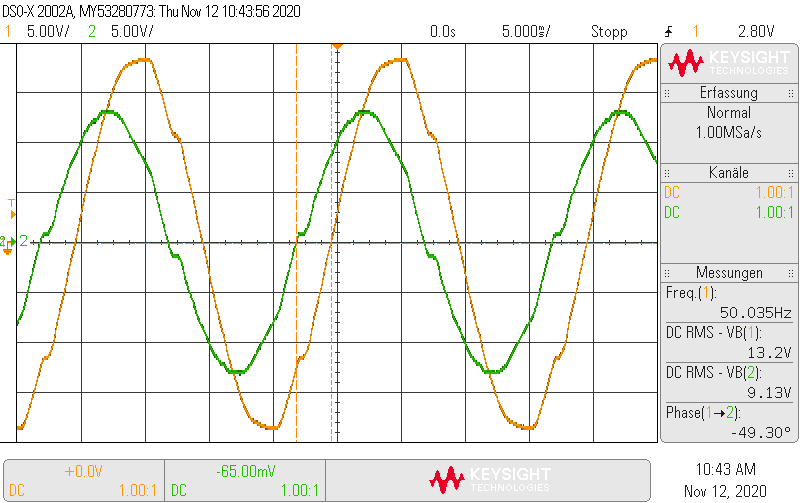
\includegraphics[scale=0.4]{daten/pul_6.png}
\end{figure}
 



\begin{figure}[H]
\centering
\caption{Spannungen in einer RL-Schaltung}
\label{fig:task5_kurve}
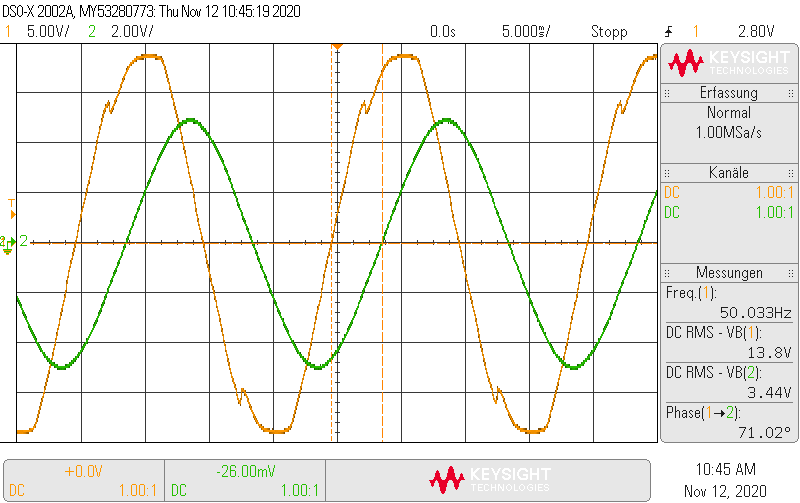
\includegraphics[scale=0.4]{daten/pul_7.png}
\end{figure}
 






\section{Auswertung}

\subsection{Untersuchung  der  Anzeige  von  unterschiedlichen  Spannungsmessinstrumenten  bei verschiedenen Kurvenformen }





Für die Effektivwerte wurde testweise eine numerische Integration durchgeführt. Hierfür wurde auf die Simpson-Formel zurückgegriffen. Diese findet sich im Python-Paket \texttt{scipy}. Im Falle der Sinus-Schwingung und der Dreiecksschwingung wurde über die eine Periode von 2 benachbarten Maxima integriert. Bei der Rechtecksschwigung wurde zwischen 2 steigenden Flanken des Rechtecks integriert. Daraus ergeben sich die Werte in Tabelle~\ref{tab:task1_num_int}.
\begin{table}[H]
\caption{Spitze-Tal Werte für die Kurven.}
\label{tab:task1_num_int}
\begin{tabular}{c|c}
Schwingung &  $U_\text{eff}$ / V  \\
\hline
Sinus &  3.557 \\
Dreieck & 2.983 \\
Rechteck & 5.487
\end{tabular}
\end{table}



Das Oszilloskop berechnet den Spitze-Tal Wert und den Effektivwert direkt. Durch Division durch den Scheitelfaktor kann man aus dem Scheitelwert den Effektivwert berechnen. Der Scheitelfaktor beträgt $\sqrt{2}$ für Sinus, $\sqrt{3}$ für Dreiecksverteilungen und $1$ für die Rechtecksverteilung. Zusätzlich muss $U_{ss}$ noch halbiert werden, damit man den Scheitelwert erhält.

\begin{table}[H]
\centering
\caption{Effektivwert mit Oszilloskop. Zum einen der gemessene Wert, zum anderen der berechnete Wert mit Hilfe des Scheitelfaktors.}
\label{tab:auswertung_task1_oszi}
\begin{tabular}{r|rrr}
 & & gemessen & berechnet \\
 Schwingung &  $U_{ss}$ / V &  $U_\text{eff}$ / V  &  $U_\text{eff}$ / V\\
\hline
Sinus & $10.15 \pm 0.20$ & $3.55 \pm 0.07$ & $3.59 \pm 0.07$ \\
Dreieck & $10.28 \pm 0.21$ & $2.97 \pm 0.06$ & $2.96 \pm 0.06$ \\
Rechteck & $11.01 \pm 0.22$ & $5.48 \pm 0.11$ & $5.51 \pm 0.11$
\end{tabular}
\end{table}





\begin{table}[H]
\centering
\caption{Gemessene Effektivwerte mit den Messgeräten P1 (MM1), P2 (MM2) und P3 (MM3) nach Grafik~\ref{fig:aufbau_task1}.}
\label{tab:auswertung_task1_volt}
\begin{tabular}{r|rrr}
& P1 & P2 & P3 \\
Schwingung & $U_{1,\text{eff}}$ / V  & $U_{2,\text{eff}}$ / V & $U_{3,\text{eff}}$ / V \\
\hline
Sinus & $3.532\pm 0.022$ & $3.535 \pm 0.028$ & $3.31 \pm 0.05$ \\
Dreieck & $2.965\pm 0.019$ & $2.863 \pm 0.024$ & $2.66 \pm 0.04$ \\
Rechteck & $5.500\pm 0.032$ & $6.003 \pm 0.040$ & $5.91 \pm 0.09$
\end{tabular}
\end{table}





\subsection{Phasenlage von Strom und Spannung an einem Kondensator bzw. einer Spule}

Die Phasenverschiebung kann theoretisch und praktisch berechnet werden. Gemäß der Formel für die Impedanz ergibt sich nach der Theorie (vgl. \cite{demtroeder})
\begin{align*}
Z_2 &= R + Z_{C_1} = R - \frac{i}{2\cdot\pi\cdot f \cdot C_1} \\
Z_3 &= R + Z_{L} = R + i\cdot 2\cdot\pi\cdot f \cdot L
\end{align*}
für die Gesamtimpedanz $Z_2$ in den Versuch 2 bzw $Z_3$ in Versuch 3.

Für die Phasenverschiebung beim Kondensator aus Aufgabe 2 ($\varphi_2$) gilt daher
\begin{align*}
\tan\left(\varphi_2\right) &= \frac{\Im(Z_2)}{\Re(Z_2)} \\
&= \frac{1}{2\cdot\pi} \cdot\left(\frac{1}{ f\cdot R \cdot C_1} \pm  \frac{\Delta f\cdot R \cdot C_1 + f\cdot \Delta R \cdot C_1 + f\cdot R \cdot \Delta C_1}{ (f \cdot R\cdot C_1)^2} \right)
\end{align*}

Für die Phasenverschiebung bei der Spule aus Aufgabe 3 ($\varphi_3$) gilt nach der Theorie
\begin{align*}
\tan\left(\varphi_3\right) &= \frac{\Im(Z_3)}{\Re(Z_3)} \\
&= 2\cdot \pi\cdot \left( \frac{f \cdot L}{R} \pm \frac{\Delta f\cdot L\cdot R + f\cdot \Delta L\cdot R + f\cdot L \cdot \Delta R}{R^2} \right)
\end{align*}


Für Aufgabe 2 ergibt sich ein theoretischer Wert $\varphi_2 = (44 \pm 8)^\circ$, die sich der Strom vor der Spannung eines Kondensators befindet. Dabei wurde allerdings von einem idealen Kondensator ausgegangen (den es real nicht gibt). Es müsste gemäß \cite{moodle} noch der Isolationswiderstand berücksichtigt werden. 

Da für die Spule keine Induktion gegeben ist, kann der theoretische Wert nicht berechnet werden.



Für die Aufgaben 2 und 3 können nun Zeigerdiagramme erstellt werden. Die Eingangsspannung ist jeweils die Summe über die Spannung am Widerstand und die Spannung am Bauteil (Kondensator bzw. Spule). Es gilt also
\begin{align*}
U_E &= U_{R1} + U_{C1}
\end{align*}
im Falle des Kondensators und 
\begin{align*}
U_E &= U_{R1} + U_{L1}
\end{align*}
im Falle der Spule.



\section{Diskussion}


\subsection{Untersuchung  der  Anzeige  von  unterschiedlichen  Spannungsmessinstrumenten  bei verschiedenen Kurvenformen }


Generell ist zu sagen, dass die meisten Messgeräte für Sinus-Schwingungen ausgelegt sind und alle anderen Schwingungen durch Sinus-Schwingungen approximieren. Durch diverse Faktoren lassen sich bekannte Funktionsverläufe ineinander umrechnen. Das funktioniert, sofern es keine gröberen Verzerrungen oder Abweichungen von der gewünschten Form gibt. Zusätzlich gelten diese Faktoren nur für definierte Signale mit einer gewissen Regelmäßigkeit. Bei sich mehrmals ändernden oder überlagerten Signalen sollte man auf numerische Integration zurückgreifen.

Wir konnten beobachten, dass das Ergebnis der numerischen Integration den Effektivwert genauer bestimmt, als der Weg über den Scheitelwert. Die Simpson-Formel für die numerische Integration liefert nach den Erkentnissen der numerischen Analysis hervorragende Werte, insbesondere für Sinusschwingungen. Es liegt daher der Schluss nahe, dass das Oszilloskop intern ebenfalls eine numerische Integration durchführt.

Es sollte zusätzlich noch kritisch hinterfragt werden, ob sich die Messgeräte bei gleichzeitiger Messung gegenseitig beeinflussen. Bei der Spannungsmessung sollte ein Messgerät über einen sehr hohen Innenwiderstand verfügen. Durch die parallelen Messungen werden diese Innenwiderstände parallel geschalten, was eine Senkung des Gesamtwiderstandes zur Folge hat. Es wäre daher besser, die Messungen nacheinander anstatt parallel durchzuführen.


\subsection{Phasenlage von Strom und Spannung an einem Kondensator bzw. einer Spule}

Für den Kondensator wurde eine Phasenverschiebung von $\varphi_2 = 92.30^\circ$ gemessen. Das ist nach der Theorie nicht möglich, da ein perfekter Kondensator ohne Widerstand eine Impedanz von 
\begin{align*}
Z_C = \frac{1}{i\cdot\omega \cdot C}
\end{align*}
aufweist. In der Beziehung $U=Z_C\cdot I$ entsteht dadurch eine $90^\circ$ Phasenverschiebung zwischen $I$ und $U$. Der Isolationswiderstand, welcher in \cite{moodle} beschrieben ist, würde diese Phasenverschiebung höchstens verkleinern. Der theoretische Wert der Phasenverschiebung wäre $\varphi_2 = (44\pm8)^\circ$ unter Vernachlässigung des Isolationswiderstandes und der Annahme eines perfekten Kondensators für die gegebenen Werte $R = 68~\Omega$, $f=50~$Hz und $C=47~\mu$F.

~

Die Impedanz einer Spule wäre 
\begin{align*}
Z_L = i\cdot\omega \cdot L
\end{align*}
Analog könnte man bei gegebener Induktivität einen theoretischen Wert für die Phasenverschiebung berechnen, sofern $L$ gegeben wäre. Die Phasenverschiebung würde sich durch das Vorzeichen von jener beim Kondensator unterscheiden.


\subsection{Leistung einer RC- bzw RL-Schaltung}

Die Leistung wird einmal durch ein Wattmeter gemessen und einmal durch manuelles Messen der Phasenverschiebung, des Stromes und der Spannung. Grundsätzlich sollte man dasselbe Ergebnis erhalten. Das Problem ist allerdings, dass hier von sämtlichen Messgeräten verschiedene Innenwiderstände überlagert werden.  Da jedes Messgerät die Messgröße geringfügig belastet, wäre hier zu klären, ob man bei einzelnen Messungen ein genaueres Messergebnis erhält. 



\section{Zusammenfassung}

\subsection{Untersuchung  der  Anzeige  von  unterschiedlichen  Spannungsmessinstrumenten  bei verschiedenen Kurvenformen }






\subsection{Phasenlage von Strom und Spannung an einem Kondensator bzw. einer Spule}


\subsection{Leistung einer RC- bzw RL-Schaltung}




\begin{thebibliography}{9}
\bibitem{moodle} Moodle-Unterlagen zum Versuch, bereitgestellt von der Karl-Franzens-Universität Graz.
\bibitem{src2} \url{https://www.spektrum.de/lexikon/physik/wechselstrom/15456}
\bibitem{src3} \url{https://www.leifiphysik.de/elektrizitaetslehre/wechselstromtechnik/grundwissen/effektivwerte-von-wechselstrom-und-spannung}
\bibitem{src4} \url{https://www.lernhelfer.de/schuelerlexikon/physik-abitur/artikel/wechselspannung-und-wechselstrom}
\bibitem{src5} \url{https://www.chemie-schule.de/KnowHow/Gleichrichtwert}
\bibitem{src6} \url{https://www.emf.ethz.ch/emf-info/themen/physik/verknuepfung-von-elektrischen-und-magnetischen-feldern/wirkleistung-blindleistung-scheinleistung/}

\bibitem{demtroeder} W. Demtröder: \emph{Experimentalphysik 2 - Elektrizität  und Optik}, 7. Auflage, 2017.

\bibitem{oszi_datenblatt} \url{https://www.keysight.com/at/de/assets/7018-02733/data-sheets/5990-6618.pdf}
\end{thebibliography}


%\newpage 
%\appendix
%\section{Python Skript}



%\lstinputlisting[language=Python,captionpos=b, label=lst:test,caption={Python Skript}]{plot.py}

%\lstinputlisting[language=Python,captionpos=b, label=lst:test,caption={Bessel Auswertung}]{generate_numbers_bessel.py}


%\lstinputlisting[language=Python,captionpos=b, label=lst:test,caption={Zerstreuungslinse Auswertung}]{generate_numbers_zerstreuungslinse.py}


\end{document}
